%%%%%%%%%%%%%%%%%%%%%%%%%%%%%%%%%%%%%%%%%%%%%%%%%%%%%%%%%%%%%%%%%%%%%%%%%%%  BASIC  %%%%%%%%%%%%%%%%%%%%%%%%%%%%%%%%%%%%%%%%%%%%%%%%%%%%%%%%%%%%%%%%%%%%%%%%%%%

\section{Basic}

\subsection{Default code}
\lstinputlisting{basic/Default.cpp}

\subsection{Misc}
\lstinputlisting{basic/Misc.cpp}

\subsection{Fast read \& write}
\lstinputlisting{basic/FastRW.cpp}

\subsection{Sort cmp}
\lstinputlisting{basic/Cmp.cpp}

\subsection{Custom unordered_map}
\lstinputlisting{basic/CustomUnordered\_map.cpp}

\subsection{字典序a嚴格小於b}
\lstinputlisting{basic/LexicographicallySmaller.cpp}

\subsection{Radom}
\lstinputlisting{basic/Radom.cpp}

%%%%%%%%%%%%%%%%%%%%%%%%%%%%%%%%%%%%%%%%%%%%%%%%%%%%%%%%%%%%%%%%%%%%%%%%%%%  Matching  %%%%%%%%%%%%%%%%%%%%%%%%%%%%%%%%%%%%%%%%%%%%%%%%%%%%%%%%%%%%%%%%%%%%%%%%%%%
\section{Matching}

\subsection{run.bat}
\lstinputlisting{matching/run.bat}

\subsection{run.sh}
\lstinputlisting{matching/run.sh}

%%%%%%%%%%%%%%%%%%%%%%%%%%%%%%%%%%%%%%%%%%%%%%%%%%%%%%%%%%%%%%%%%%%%%%%%%%%  Python  %%%%%%%%%%%%%%%%%%%%%%%%%%%%%%%%%%%%%%%%%%%%%%%%%%%%%%%%%%%%%%%%%%%%%%%%%%%
\section{Python}

\subsection{Decimal}
\lstinputlisting{python/Decimal.py}

\subsection{Fraction}
\lstinputlisting{python/Fraction.py}

\subsection{Misc}
\lstinputlisting{python/Misc.py}
\onecolumn
\centering
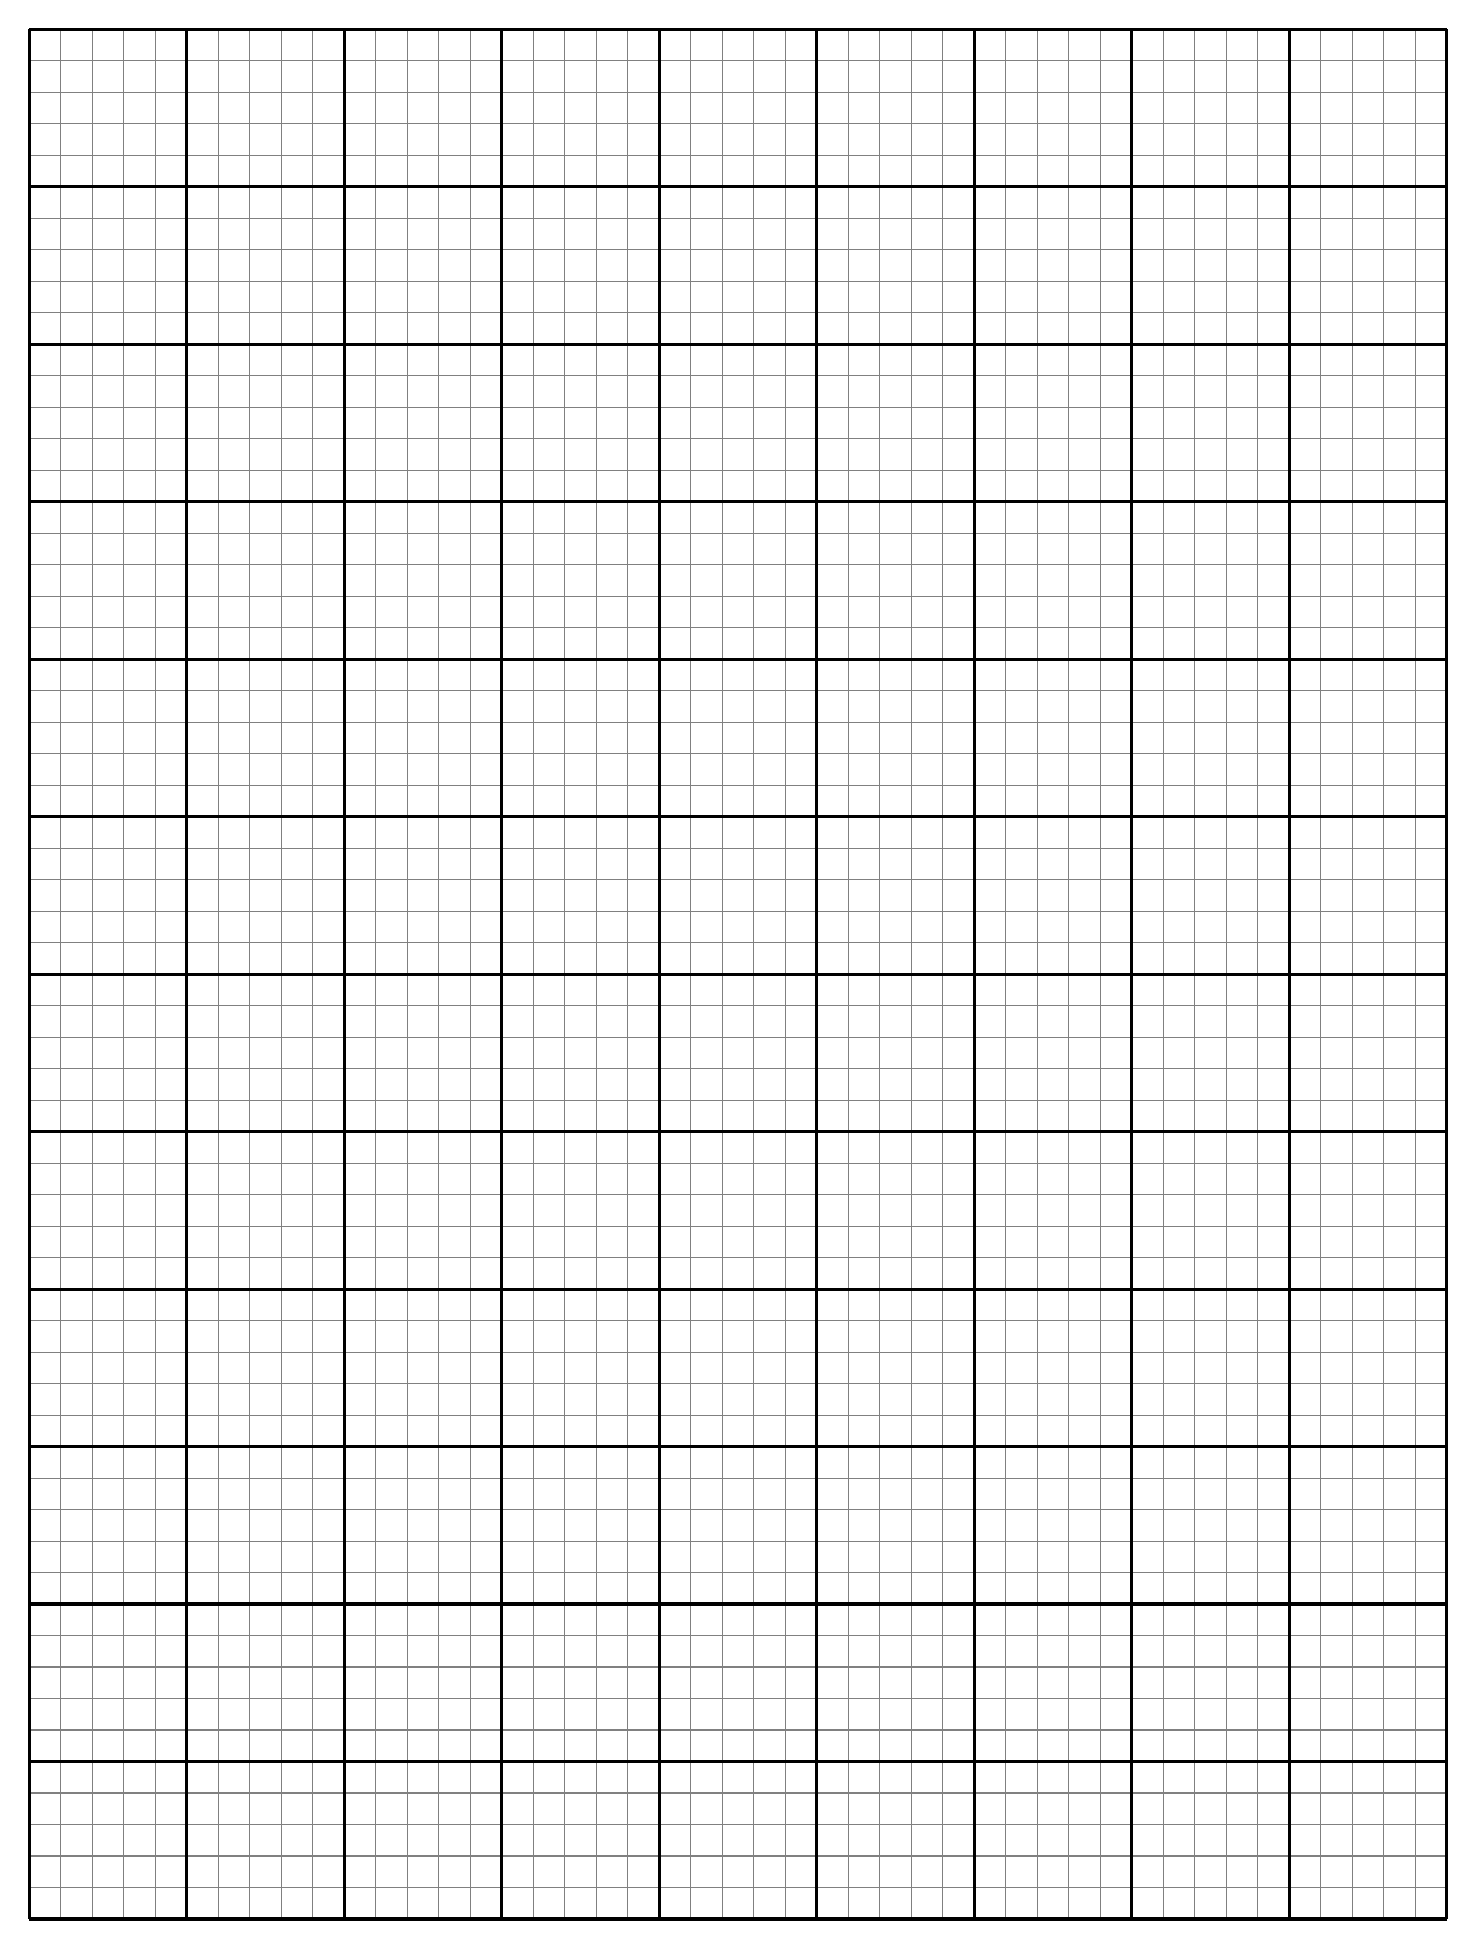
\begin{tikzpicture}[every node/.style={minimum size=1cm-\pgflinewidth, outer sep=10pt}, scale=2]
    \draw[step=0.2cm,color=gray] (0,0) grid (9,12);
    \draw[step=1cm,color=black,line width=0.4mm] (0,0) grid (9,12);
\end{tikzpicture}

\centering
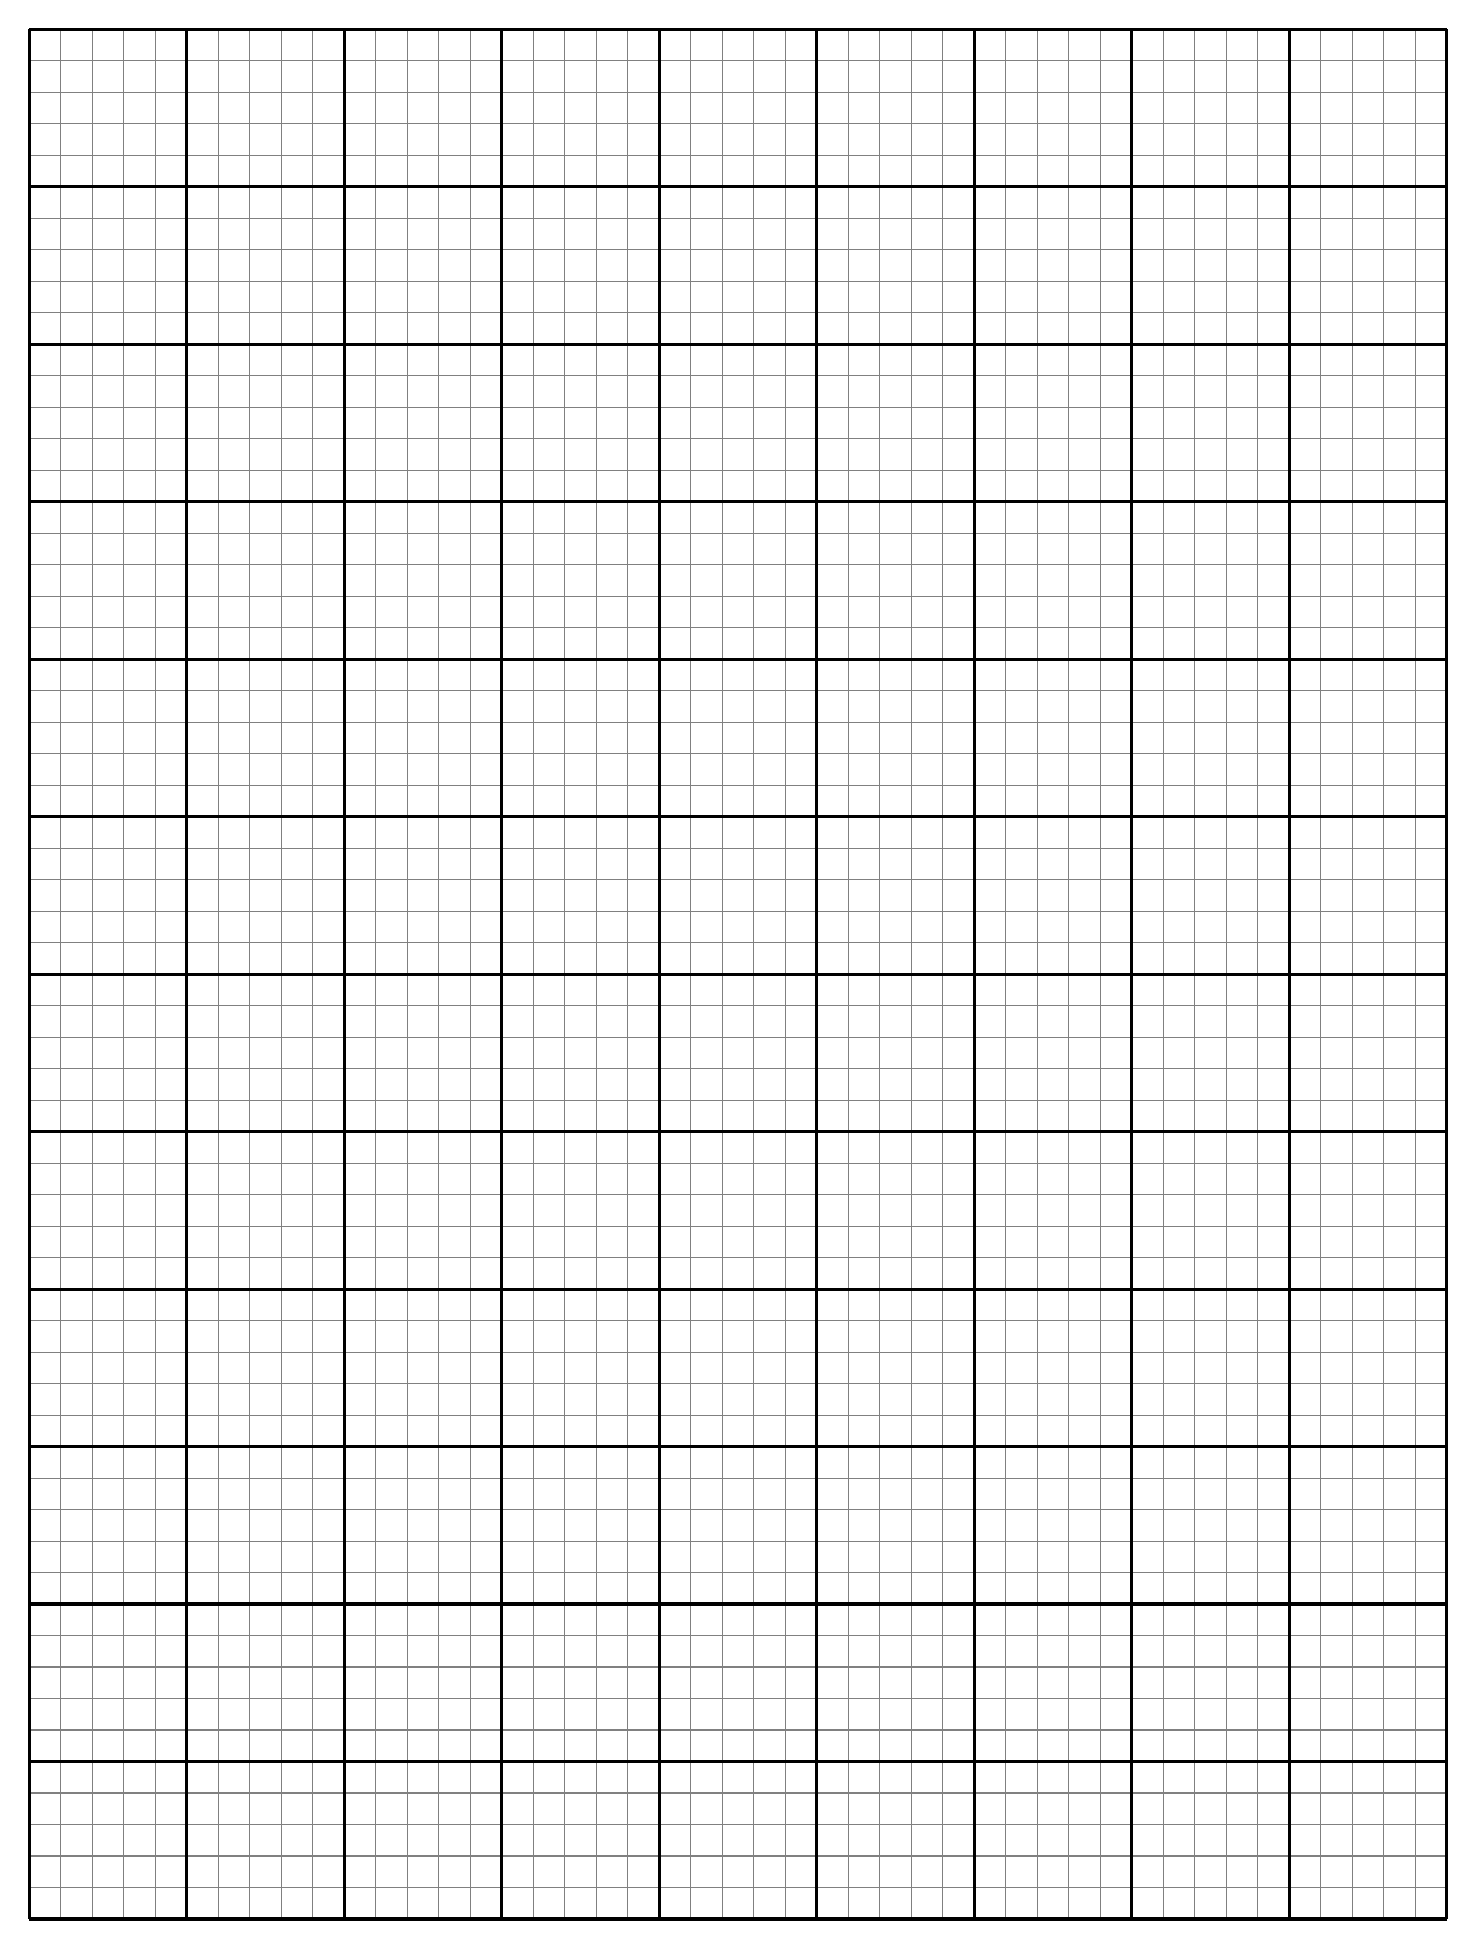
\begin{tikzpicture}[every node/.style={minimum size=1cm-\pgflinewidth, outer sep=10pt}, scale=2]
    \draw[step=0.2cm,color=gray] (0,0) grid (9,12);
    \draw[step=1cm,color=black,line width=0.4mm] (0,0) grid (9,12);
\end{tikzpicture}